\documentclass[12pt, a4paper, oneside]{ctexbook}
\usepackage{amsmath, amsthm, amssymb, bm, graphicx, hyperref, mathrsfs}

\title{{\Huge{\textbf{线性优化与凸优化笔记}}}\\为了熟悉LaTeX}
\author{Ray}
\date{\today}
\linespread{1.5}
\newtheorem{theorem}{定理}[section]
\newtheorem{definition}[theorem]{定义}
\newtheorem{lemma}[theorem]{引理}
\newtheorem{corollary}[theorem]{推论}
\newtheorem{example}[theorem]{例}
\newtheorem{proposition}[theorem]{命题}
\newtheorem{fomula}[theorem]{公式}

\begin{document}

\maketitle

\pagenumbering{roman}
\setcounter{page}{1}

\begin{center}
    \Huge\textbf{前言}
\end{center}\

这是笔记的前言部分. 

\begin{flushright}
    \begin{tabular}{c}
        Dylaaan\\
        \today
    \end{tabular}
\end{flushright}

\newpage
\pagenumbering{Roman}
\setcounter{page}{1}
\tableofcontents
\newpage
\setcounter{page}{1}
\pagenumbering{arabic}

\chapter{数学基础知识}

这一章主要讲的是数学的基本知识，对以后的学习\textbf{很重要！} 

\section{优化问题示例：SVM}
一般写作$\min_{x\in X}f(x)$，意思是在$x$属于$X$的条件下，$f(x)$的最小值。
\begin{enumerate}
    \item 一些重要参数的名字 \\
$f$:目标函数(objective function) \\ $x$:决策变量(decision variable) \\ $X$:约束集(constrain set)

    \item 支持向量机(SVM)简述 \\
它是要寻找特殊空间中的线性分类器。
SVM学习的基本想法是求解能够正确划分训练数据集并且找到几何间隔最大的分离超平面。

    \item 目标 \\
给定n个数据点$(x_i,y_i)$，其中$x_i$是空间中的坐标，$y_i$代表不同的两类，分别是1或-1。
我们需要找到一个线性分类函数$f(x)=w^Tx+b$，使得$y_if(x_i)>0$，也就是将其分为两类，
而且要最大化这个线性函数到所有数据点的最小值。写成优化问题的格式，就是：
$$\max_{w,b}\min \frac{|w^T\cdot x_i+b|}{||w||}$$
$$s.t.\text{ }y_i(w^Tx_i+b)>0$$

    \item 化简 \\
首先令$w'=\alpha w$，$b'=\alpha b$，可知形式不变（即具有齐次性）。所以我们可以选取适当
的$\alpha$，让$\min|w^T\cdot x_i+b| = 1$。\\ 再将$\max_{w,b}\frac{1}{||w||}$变为
$\min_{w,b}\frac{1}{2}||w||^2$，即可得到最终形态：
$$\min_{w,b}\frac{1}{2}||w||^2$$
$$s.t. \text{ }y_i(w^Tx_i+b)>1$$

\end{enumerate}
\section{多元、多个函数运算}
\begin{enumerate}

    \item 导数（derivative）
一元函数：$f'(x_0) = Df(x_0) = A$

多个多元函数：Jacobian matrix of $f=(f_1,\dots,f_m)$

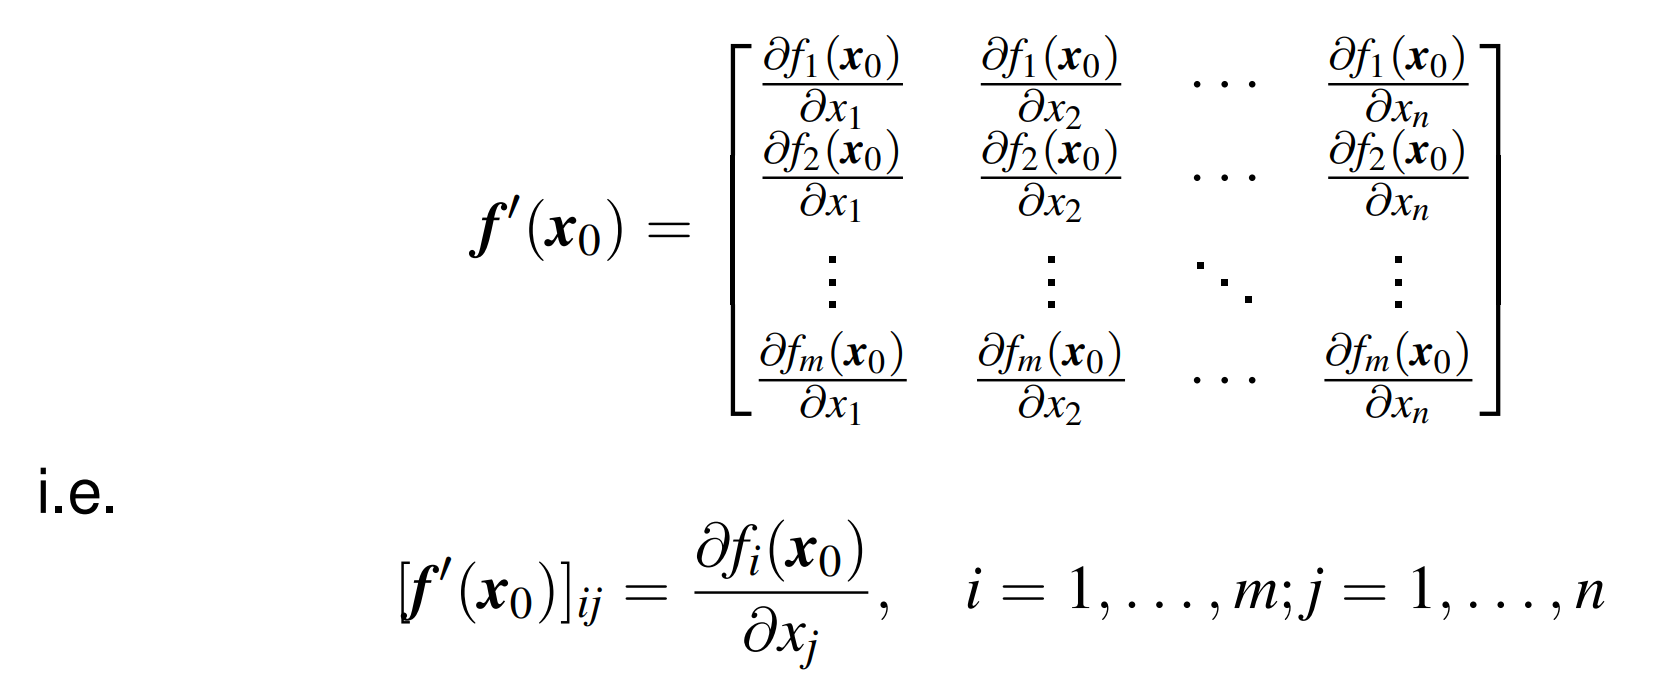
\includegraphics[scale=0.5]{figures/屏幕截图 2023-09-20 232328.png}

所以
$$
f_i(x_0+\Delta x)=f_i(x_0)+\sum_{j=1}^{n}\frac{\partial f_i(x_0)}{\partial x_j}\Delta x_j+o(\Delta x)
$$

\begin{example}
    对称矩阵$A$，$f(\vec x)=x^TAx=\sum_{i=1}^{n}\sum_{j=1}^{n}A_{ij}x_ix_j$对$x$的导数为
    $$f'(x)=2x^TA$$
\end{example}

\begin{proof}
    $$
    f(x_0)+\Delta x-f(x_0)=x_0^T(A+A^T)\Delta x+\Delta x^TA\Delta x
    $$
\end{proof}
\begin{corollary}
    对于一般的矩阵$A$，有$f'(x)=\frac{1}{2}(A+A^T)$
\end{corollary}

    \item 梯度（gradient）定义为它的导数矩阵的转置。$\nabla f(x)=[f'(x)]^T$

\begin{proposition}
    对于对称矩阵$A$，$f(x)=x^TAx+b^Tx+x$的梯度为
    $$
    \nabla f(x) = 2Ax+b
    $$
    由例1.1.1得到的结果转置而来。
\end{proposition}

\begin{lemma}
    向量$\vec x$一般是n行1列的类型，所以$\vec a\cdot \vec b=\vec a^T \vec b$，
    而$f'(\vec x)$是一个1行n列的向量，$\nabla f(\vec x)$则是$f'(\vec x)$的转置，即为n行1列的向量。
\end{lemma}

    \item 链式法则

涉及到向量、矩阵相乘的函数，链式法则会相应的有所变化，具体请看下面一些例子。
\begin{example}
    已知$h(\vec x) = f(A\vec x+\vec b)$，求$h'(\vec x_0)$和$\nabla h(\vec x_0)$.
\end{example}
\begin{proof}
    根据$A->(m,n)$，$x->(n,1)$，可以得到 \\
    $h'(x_0)=f'(Ax_0+b)A$——————(左右矩阵的大小一样) \\
    所以由于梯度与导数的关系，有
    $$\nabla h(x_0) = A^T(f'(Ax_0+b))^T = A^T\nabla f(Ax_0+b)$$
\end{proof}

    \item 二阶导数、二阶梯度

\begin{example}
    对称矩阵$A$，$f(\vec x)=x^TAx=\sum_{i=1}^{n}\sum_{j=1}^{n}A_{ij}x_ix_j$对$x$的二阶梯度为
    $$\nabla ^2f(\vec x)=2A$$
\end{example}

\begin{proof}
    根据例1.1.1，$\nabla f(\vec x)=2A\vec x$，

    所以$\nabla f^2(\vec x)=D(\nabla f(\vec x))=D(2A\vec x)=2A$
\end{proof}

\begin{example}
    是例1.2.5的后续：已知$h(\vec x) = f(A\vec x+\vec b)$，求$\nabla^2 h(\vec x)$.
\end{example}

\begin{proof}
    为方便理解，记$y=Ax+b$. 接着一层一层来：由1.2.5知
    $\nabla h(x)=A^T \nabla h(y)$，然后再来一层：
    $$\nabla^2 h(\vec x)=D_x(\nabla h(x))=D_x(A^T \nabla h(y))=A^T D_x(\nabla h(y))$$
    $$=A^T D_y(\nabla h(y))D_xy=A^T\nabla^2h(y)A$$.
\end{proof}

    \item 矩阵的（半）正定和（半）负定 \\
这里将给出矩阵判断（半）正、负定的一种方法：主子式法。
\begin{theorem}
    矩阵$A$正定 $\leftrightarrow$ $A$的顺序主子式的值都$>0$. 
\end{theorem}

\begin{theorem}
    矩阵$A$半正定 $\leftrightarrow$ $A$的主子式的值都$\geq 0$. 
\end{theorem}

\begin{theorem}
    矩阵$A$负定 $\leftrightarrow$ $-A$的顺序主子式的值都$>0$. 
\end{theorem}


\chapter{凸集}

\section{凸集的定义和一些凸集}
\begin{definition}
    集合C是凸集当且仅当对任意$x,y\in C$，$\theta \in [0,1]$，有
    $$\theta x+(1-\theta)y\in C.$$
\end{definition}

\begin{example}
    几种常见的凸集： \\
    1. 超平面$P=\{x\in R^n:w^Tx=b\}$是凸集，对$w\in R,b\in R.$ \\
    2. 半空间$P=\{x\in R^n:w^Tx\leqslant b\}$是凸集，对$w\in R,b\in R.$ \\
    3. 两个凸集的交集是凸集。 \\
    4. 仿射空间$S=\{x\in R:Ax=b\}$是凸集，$A\in R^{m*n},b\in R^m.$ \\
    5. 多边形$P=\{x\in R^n:Ax\leqslant b\}$是凸集，对$A\in R^{m*n},b\in R^m.$ \\
    6. 单位球$B(x_0,r)=\{x\in R^n:||x-x_0||\leqslant r\}$是凸集。（对任意范式$||.||$都成立）\\
    7. 椭圆$\epsilon=\{x\in R^2:\frac{x_1^2}{\lambda_1^2}+\frac{x_2^2}{\lambda_2^2}\leqslant 1\}$是凸集。\\
    8. 仿射椭圆$\epsilon=\{x_0+Au:||u||_2\leqslant 1\},A\in R^{n*n},A$正定是一个凸集。\\
    9. 仿射变换下的凸集还是一个凸集。 \\
    10.抽象集合$S^n_+=\{A\in R^{n*n}:\text{A是半正定矩阵}\}$是凸集。\\
\end{example}

\section{凸集上的投影}
    对于某个点x，凸集C与x的距离为$dist(x,C)=inf_{z\in C}||x-z||.$ \\
    对任意的x，凸集中存在一个唯一的点$\hat{x}$，使$dist(x,C)=||x-\hat{x}||.$ \\
    这个点被记作$\hat{x}=P_c(x).$

\begin{proposition}
    对非空闭集凸集$C$，$\hat{x}=P_C(x)$当且仅当对任意$z\in C$，$\left \langle x-\hat{x},z-\hat{x}\right \rangle \leqslant 0.$
\end{proposition}
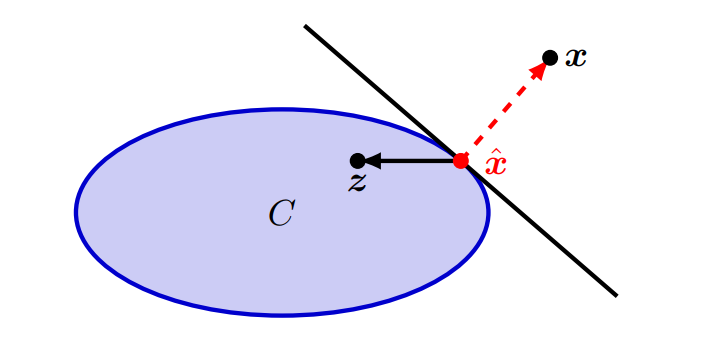
\includegraphics[scale=0.8]{figures/屏幕截图 2023-10-14 110753.png}

\begin{proposition}
    投影运算是nonexpansive的，即$||P_C(x)-P_C(y)||\leqslant||x-y||.$ \\
    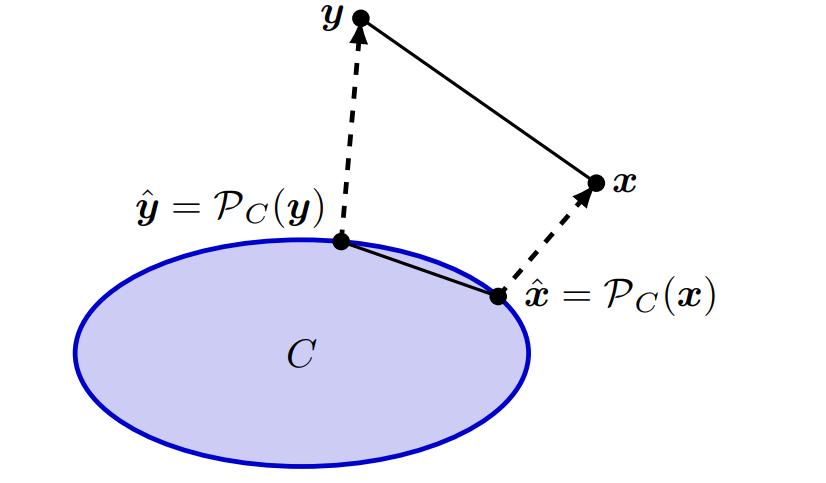
\includegraphics[scale=0.8,height = 5cm, width = 9cm]{figures/屏幕截图 2023-10-14 111403.png}
\end{proposition}

\begin{proposition}
    对闭合非空凸集C，对$x_0\notin C$，存在$w$，使得$sup_{x\in C}\left \langle w,x\right \rangle < \left \langle w,x_0\right \rangle.$ \\
    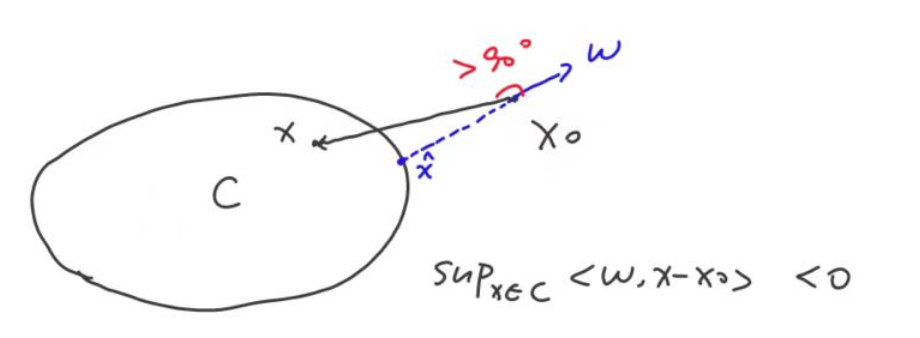
\includegraphics[scale=0.8,height = 4cm, width = 10cm]{figures/屏幕截图 2023-10-14 112553.png}
\end{proposition}

\begin{proposition}
    集合$C$的边界记作$\partial C=\overline{C} \text{或者} int C.$ \\
    \textbf{支撑超平面定定理}： \\
    对非空凸集$C$，$x_0\in \partial C$，存在方向$w$，使得$\left \langle w,x\right \rangle < \left \langle w,x_0\right \rangle.$
    其中$P=\{x:w^Tx=w^Tx_0\}$叫做支撑超平面。 \\
    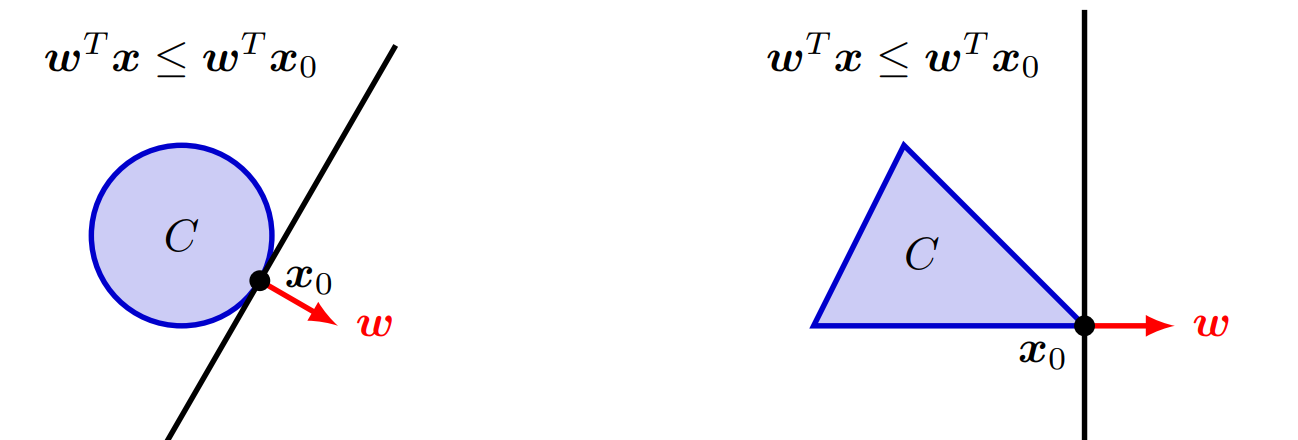
\includegraphics[scale=0.6]{figures/屏幕截图 2023-10-14 113806.png}
\end{proposition}

\begin{proposition}
    \textbf{分割超平面定理}：如果$C_1,C_2$是不相交的非空凸集，则$C_1,C_2$可以被一个超平面分成两部分，
    也就是说存在方向$w,b$使得
    $$w^Tx\leqslant b,\forall x \in C_1$$
    $$w^Tx\geqslant b,\forall x \in C_2$$
    $P=\{x:w^Tx=b\}$叫做$C_1,C_2$的分割超平面。 \\
    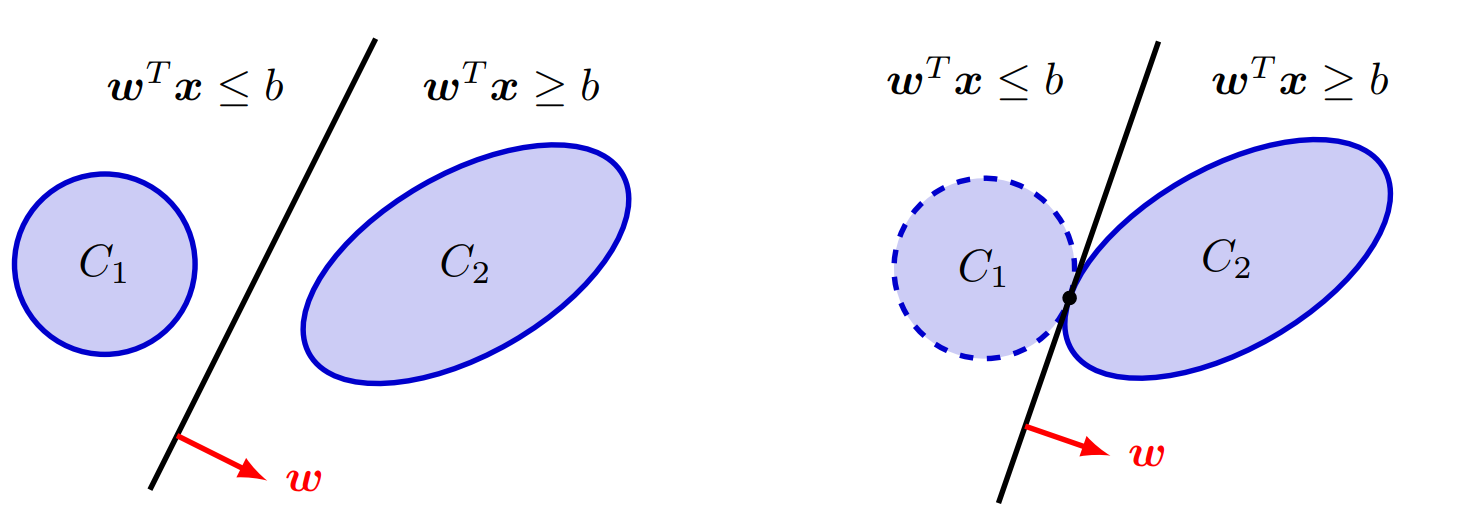
\includegraphics[scale=0.5]{figures/屏幕截图 2023-10-14 114533.png}
\end{proposition}
\end{enumerate}


\chapter{凸函数}

\section{凸函数的定义与性质}
定义：一个函数f是凸函数当且仅当定义域$domf$是凸集且对任意$x,y,\theta\in [0,1]$，
成立$$f(\theta x+\overline{\theta}y)\leqslant\theta f(x)+\overline{\theta}f(y).$$

\begin{proposition}
    $f$是凸集当且仅当对任意$x\in domf$和任意的方向$d$，函数$g(t)=f(x+td)$是凸函数。
\end{proposition}

\begin{proposition}
    定义$f$的拓展函数$$f(x)=\begin{cases}
        \tilde{f}(x)& x \in S\\
        +\infty& x \notin S 
        \end{cases},$$
    $f$为凸函数当且仅当$\tilde{f}$为凸函数。
\end{proposition}


\section{凸函数的一阶导数}
\begin{theorem}
    一个定义域是凸集的函数$f$是（严格）凸函数当且仅当对任意$x,y\in domf,$$$f(y)\geqslant (>)f(x)+\nabla f(x)^T(y-x).$$
\end{theorem}

\begin{theorem}
    定义在$I$上的映射$f$是（严格）凸函数当且仅当$f'$在$I$上（严格）递增。
\end{theorem}
\begin{proposition}
    如果对凸函数$f$，$\nabla f(x^*)=0$，则$x^*$是一个全局最小值。如果f是严格凸函数，则$x^*$是唯一的全局最小值。
\end{proposition}

\section{凸函数的二阶导数}
\begin{theorem}
    二阶可导的函数$f$是凸函数当且仅当对任意的$x$，$f''(x)\geq0.$
\end{theorem}
\begin{theorem}
    当对任意$x$，$\nabla^2f(x)$是正定的，则定义在凸集上的二阶可导函数$f$是严格凸函数。（反之不成立，考虑$f(x)=x_1^4+x_2^2$在$(0,0)$）
\end{theorem}

\begin{example}
    对数和函数$f(\vec x)=log(\sum_{i=1}^{n}e^{x_i})$是凸函数。
\end{example}

\section{凸函数的性质}
下水平集:$C_\alpha=\{x\in domf:f(x)\leq \alpha\}$. \\
上镜图：$epif=\{(x,y)\in R^{n+1}:x\in S,y\geq f(x)\}$，也就是函数的上部分。
\begin{proposition}
    f是定义在S上的凸函数，如果$x^*$是f的局部最小值，则它就是f在S上的全局最小值。
\end{proposition}
\begin{proposition}
    对严格凸函数来说，全局最小值点的个数不超过一个。
\end{proposition}
\begin{proposition}
    凸函数的下水平集是一个凸集。\\
    一些例子：\\
    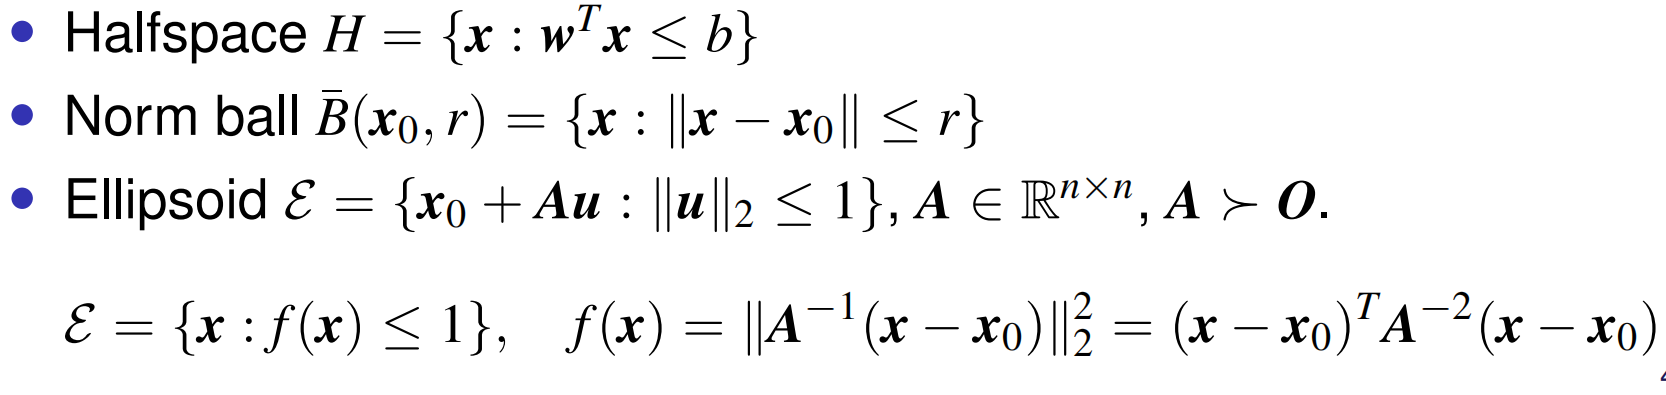
\includegraphics[scale=0.5]{figures/屏幕截图 2023-10-22 140639.png}
\end{proposition}

\begin{theorem}
    f是凸函数当且仅当epif是凸集。
\end{theorem}
\begin{theorem}
    琴生不等式：

    {\centering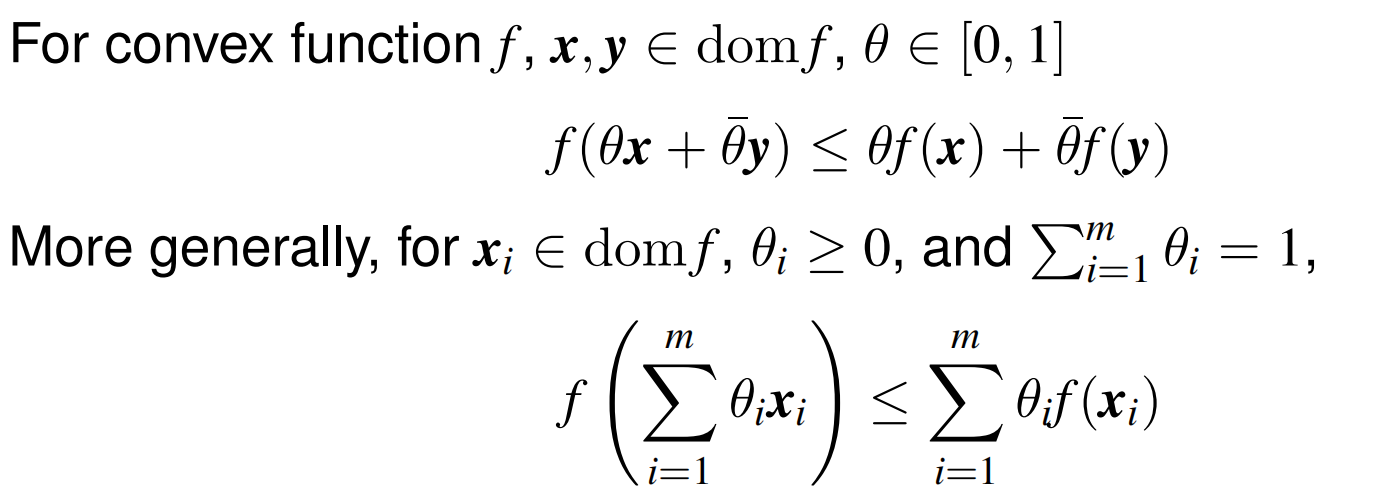
\includegraphics[scale=0.5]{figures/琴生不等式.png}

    }
\end{theorem}
\begin{theorem}
    赫尔德不等式：\\
    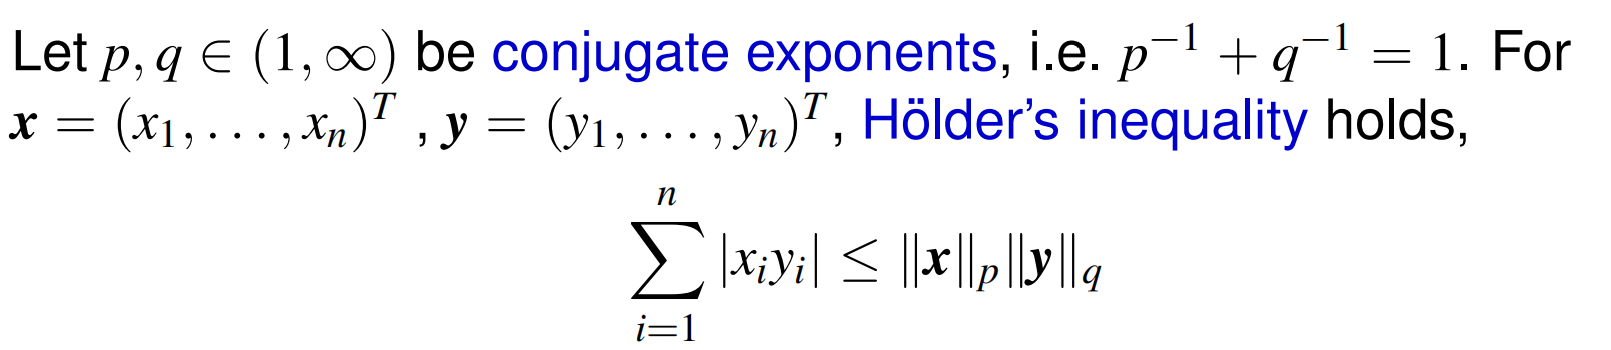
\includegraphics[scale=0.5]{figures/赫尔德不等式.png}
\end{theorem}

\subsection{凸函数的运算}
\begin{proposition}
    设$f_i$是凸函数，则对任意$c_i\geq0$，函数$f=\sum_{i=1}^{m}c_if_i(x)$是凸函数。
\end{proposition}

\begin{proposition}
    $g$为凸函数，则$f=g(Ax+b)$也是凸函数。\\
    例1. $f(x)=\|Ax-y\|$是凸函数。 \\
    例2. $f(x)=\log(\sum_{i=1}^{n}e^{w_i^T+b_i})$是凸函数.
    考虑$g(y)=\log(\sum_{i=1}^{n}e^y_i)$ 且 $y=[w_1,...,w_n]^Tx+b.$
\end{proposition}
\begin{proposition}
    复合函数性质：\\
    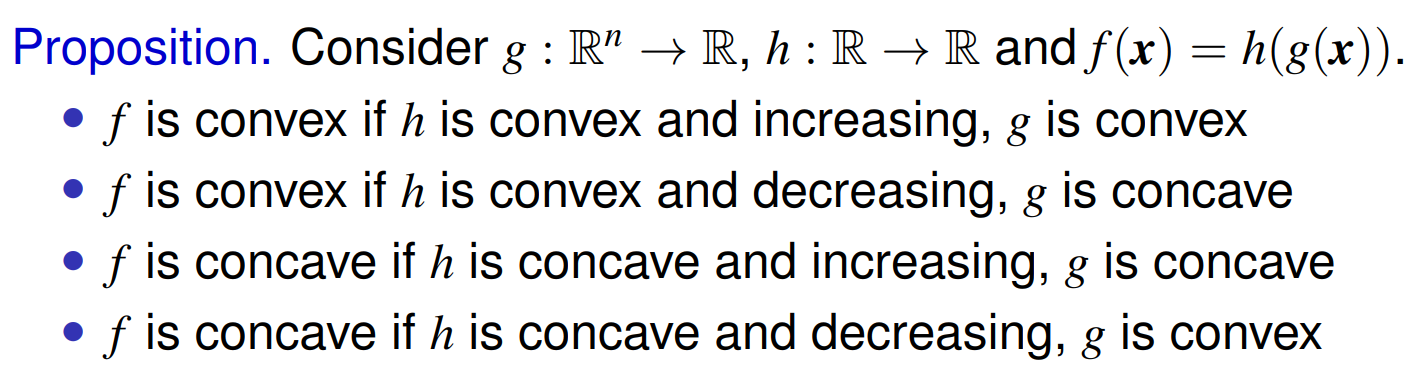
\includegraphics[scale=0.6]{figures/复合函数.png}
\end{proposition}

\begin{proposition}
    设$f_i$是凸函数，$i=1,2,...,m.$则$f(x)=\max_{1\leq i\leq m}f_i(x)$是凸函数。
\end{proposition}
\begin{proposition}
    设$f_i, i\in I$是凸函数，则$f(x)=\sup_{i\in I}f_i(x)$是凸函数。 \\
    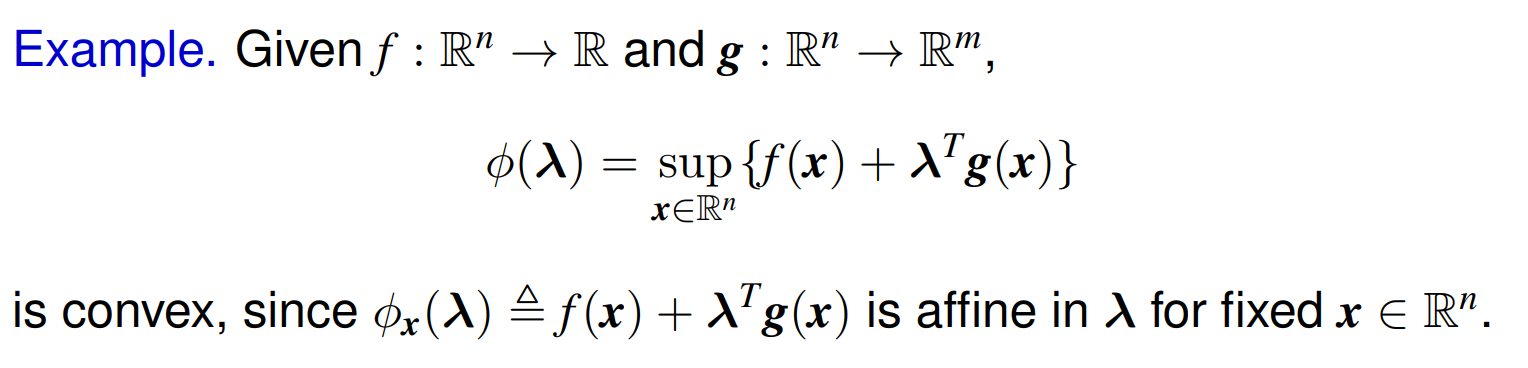
\includegraphics[scale=0.5]{figures/凸函数.png}
\end{proposition}

\begin{proposition}
    部分最小值：设$g(x,y)$是凸函数，C是凸集，则$f(x)=\inf_{y\in C}g(x,y)$是凸函数。\\
    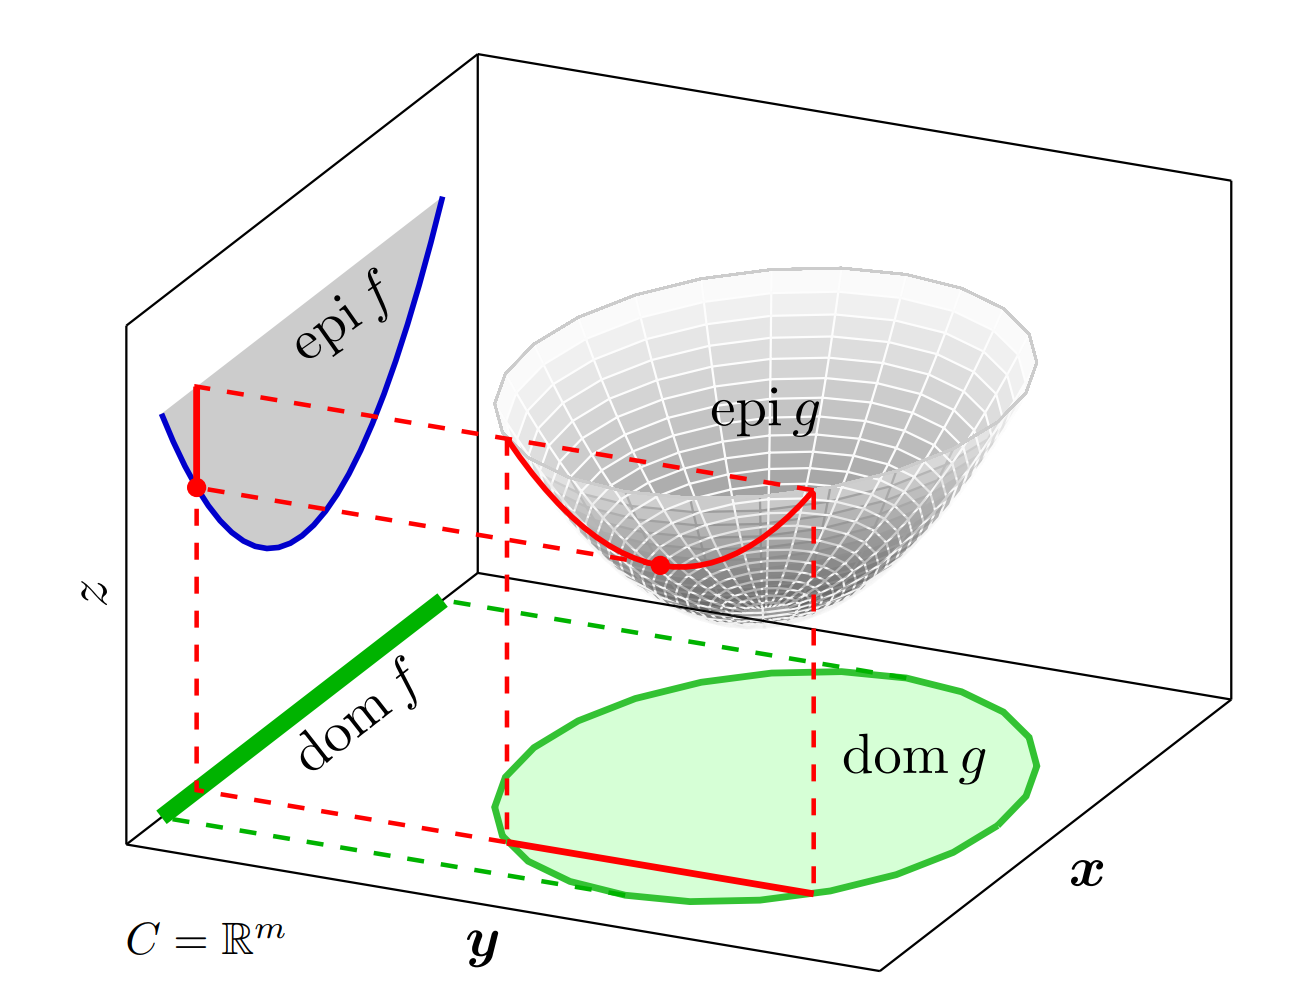
\includegraphics[scale=0.4]{figures/凸函数2.png} \\
    例：到凸集的距离函数是凸函数，即$dist(x)=\inf_{y\in C}\|x-y\|$是凸函数. \\
    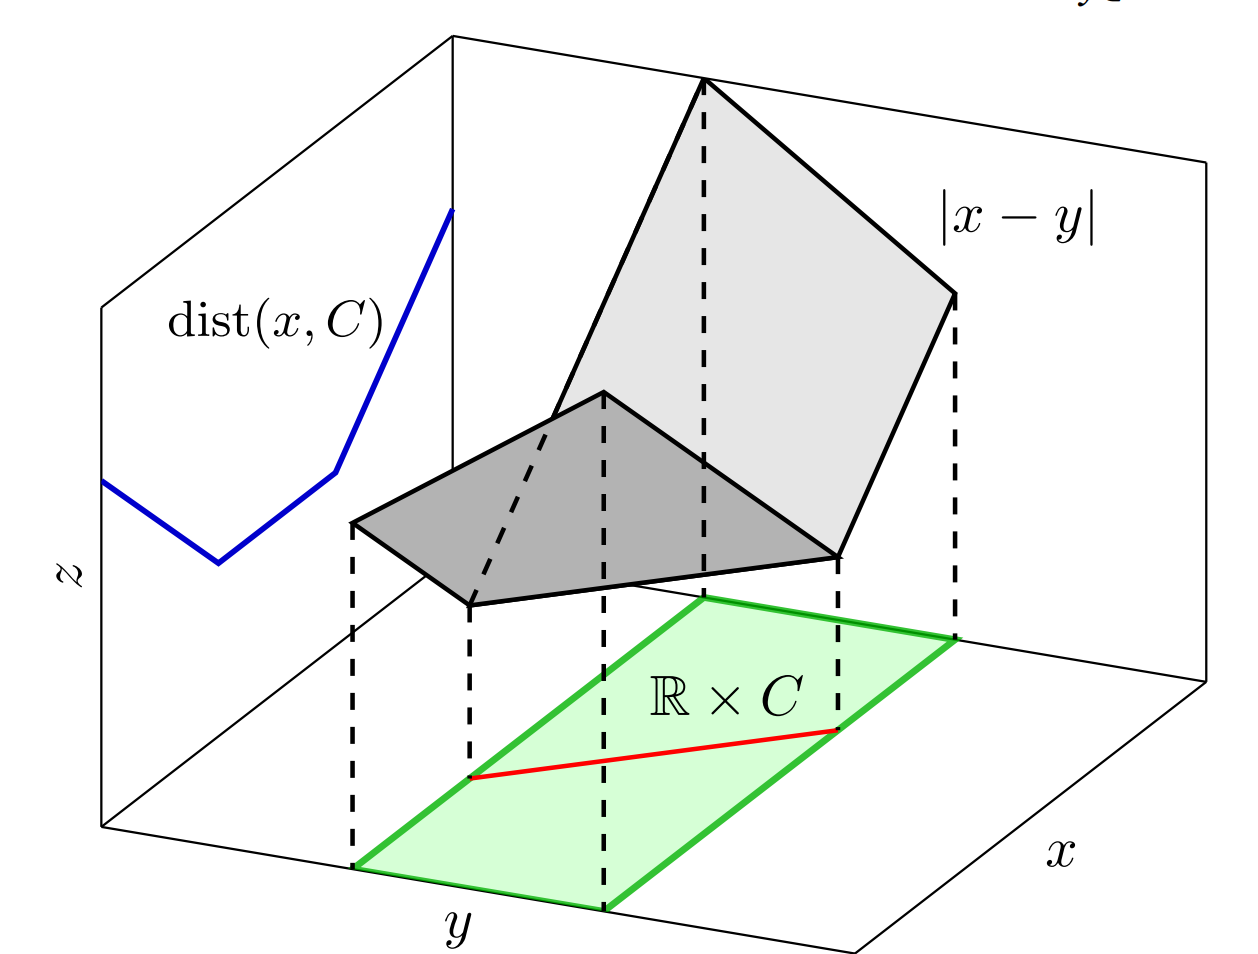
\includegraphics[scale=0.4]{figures/凸函数3.png}
\end{proposition}

\chapter{凸优化问题（部分1）}
\section{凸优化问题}
标准形式:
\begin{equation*}
    \begin{split}
    &\min_x \,f(x)\\
    &s.t.\quad  \left\{\begin{array}{lc}
        g_i(x)\leq 0,\, i=1,2,...,m\\
        h_i(x)=0,\, i=1,2,...,k\\
    \end{array}\right.
    \end{split}
\end{equation*}
\begin{itemize}
    \item $x$: 优化/决策变量
    \item $f$: 目标函数
    \item $g_i$: 不等约束条件
    \item $h_i$: 等式约束条件
    \item 可行域$X=\{x\in D:g_i(x)\leq0, 1\leq i\leq m;h_i(x)=0,i\leq i\leq k\}$.
    问题P可行当且仅当$X\neq\emptyset.$
    \item 最优值：$f^*=\inf_{x\in X}f(x).$
    \item 最优点: $x^*\in X$且$f^*=f(x^*).$
    \item $\epsilon-$次优点：$x_0\in X$且$f(x_0)\leq f^*+\epsilon.$
    \item 局部最优解: 增加限制$\|x-x^*\|\leq \delta$的P的解。
\end{itemize}
\begin{proposition}
    它是凸优化问题当且仅当\\
    1. $f,g_i$是凸函数，\\
    2. $h_i$是仿射函数，即$h_i(x)=a_i^Tx-b.$
\end{proposition}

\begin{proposition}
    对凸优化问题来说，
    \begin{itemize}
        \item 解集是凸集，$X_{opt}=\{x^*\in X:f(x^*)\leq f(x),\forall x\in X\}.$
        \item 任何局部最优解就是全局最优解。
        \item 如果$f$是严格凸函数，则最多只有一个解，$\|X_{opt}\|\leq1.$
    \end{itemize}
\end{proposition}

\begin{theorem}
    一阶最优条件：对于凸优化问题且目标函数$f$可以一阶导的情况下，可行点$x^*\in X$是最优的当且仅当
    $$\nabla f(x^*)^T(x-x^*)\geq 0.$$
\end{theorem}
\end{document}